\documentclass[a4paper,12pt]{article}
\usepackage{geometry}
\geometry{left=2.5cm,right=2.5cm,top=2.5cm,bottom=2.5cm}
\renewcommand{\textfraction}{0.15}
\renewcommand{\topfraction}{0.85}
\renewcommand{\bottomfraction}{0.65}
\renewcommand{\floatpagefraction}{0.60}
\usepackage{amsmath}
\usepackage{amsfonts}
\usepackage{mathrsfs}
\usepackage{amsthm}
\usepackage{extarrows}
\usepackage{bm}
% \newcommand{\bm}{\symbfit}    % `bm` confilicts with `unicode-math`. In that case use \symbfit for bold math symbols
\usepackage{graphicx}
\usepackage[section]{placeins}
\usepackage{flafter}
\usepackage{array}
\usepackage{caption}
\usepackage{subcaption}
\usepackage{color}
\usepackage{multirow}
\usepackage{natbib}
% \usepackage{enumerate}
\usepackage{enumitem}    % more flexible than `enumerate` package, the reference will carry the whole label appearance, not just the counter, unlike the `enumerate` package.
\usepackage{upgreek}    % 'upgreek' letters

% \pdfstringdefDisableCommands{\let\bm=\relax}

\newtheorem{thm}{Theorem}
\newtheorem{cor}{Corollary}
\newtheorem{assum}{Assumption}
\newtheorem{rem}{Remark}
\newtheorem{lem}{Lemma}
\newtheorem{prop}{Proposition}

\setcounter{topnumber}{5}    % Maximum number of floats that can appear at the top of a text page; default 2. 
\setcounter{bottomnumber}{5}   % Maximum number of floats that can appear at the bottom of a text page; default 1. 
\setcounter{totalnumber}{10}    % Maximum number of floats that can appear on a text page; default 3. 

\DeclareMathOperator*{\argmaxdown}{arg\,max}
\DeclareMathOperator*{\argmindown}{arg\,min}
\DeclareMathOperator{\argmax}{arg\,max}
\DeclareMathOperator{\argmin}{arg\,min}

% cross-reference to other files
% the externaldocument should be compiled 
% (and at least twice if you're using xr-hyper)
% \usepackage{xr-hyper}
% \usepackage{xr}

% --- external document (ordinary setting) ---
% \externaldocument{external_tex_file}
% --- end of ordinary setting ---

% --- external document (overleaf setting) ---
% externaldocument settings for Overleaf
% \makeatletter
% \newcommand*{\addFileDependency}[1]{% argument=file name and extension
% \typeout{(#1)}
% \@addtofilelist{#1}
% \IfFileExists{#1}{}{\typeout{No file #1.}}
% }
%   \makeatother
%   \newcommand*{\myexternaldocument}[1]{%
%   \externaldocument{#1}%
%   \addFileDependency{#1.tex}%
%   \addFileDependency{#1.aux}%
% }
%   \myexternaldocument{external_tex_file}
%   --- end of overleaf setting ---

%   mathtools can be used to define labeling format for equations
%   one can use \eqref for a reference to a labeled equation.
\usepackage{mathtools}
\newtagform{supp}{(S-}{)}    % define a equation labeling format for suppliment
\usetagform{supp}            % use the supp format
\usetagform{default}         % use the default format

\usepackage{algorithmic}
\usepackage{algorithm}
\renewcommand{\algorithmicrequire}{\textbf{Input:}}
\renewcommand{\algorithmicensure}{\textbf{Output:}}

% package for hyperlinks
% It's error-prone because hyper link is quite difficult
% due to the fact the typesetting environment is complex.
% So you can disable this package and finish the document.
% Then sort out the hyperlink thing.
\usepackage[colorlinks,linkcolor=red,anchorcolor=blue,citecolor=green,CJKbookmarks=True]{hyperref}

% package for displaying highlighted codes
\usepackage{minted}

% package for input codec and output rendering font
\usepackage[utf8]{inputenc}    % it is always good practice to use utf8
% you can also try latin1, latin2, cp1252 and cp1250
\usepackage[T1]{fontenc}    % the default is T0, which only contains 128 characters
% you can try T1, T2A, T2B
% you can refer to https://www.overleaf.com/learn/latex/international_language_support#Font_encoding
% for more details.


\title{Bayesian Concepts}
\author{Chao Cheng}
\date{\today}



\begin{document}
\maketitle
\tableofcontents{}

\section{Introduction}
\label{sec:introduction}

\begin{enumerate}
\item Prior and posterior distribution
\item Predictive probability and application in phase II design
\item Credible interval
\end{enumerate}

From the frequentist perspective, we have the data $x$ and the parameter of the distribution $\theta$ and we make estimation/inference about $\theta$. But $\theta$ is alwyas treated as a fixed parameter. But from bayesian perspective, $\theta$ is also a random variable.
First we introduce some notations:

\begin{itemize}
\item The prior distribution
  $\pi\left(\theta | \alpha\right)$, where $\alpha$ is fixed parameters for the distribution of $\theta$. This prior distribution of $\theta$ represents our previous  knowledge of $\theta$ before the data $x$ is collected.
\item The data distribution
  $f\left(x\middle|\theta\right)$, which is the same as that from frequentist's perspective.
\item The posterior distribution
  $f_{post}\left(\theta\middle| x\right)$, which is the distribution of $\theta$ based on (conditional on) the observed data. Note that
  \[
    f_{post}\left(\theta\middle| x\right)
    = \frac{f\left(\theta, x\right)}{f\left(x\right)}
    = \frac{
      f\left(x\middle|\theta\right)\pi\left(\theta\middle|\alpha\right)
    }{f\left(x\right)}
    \propto f\left(x\middle|\theta\right)\pi\left(\theta\middle|\alpha\right)
    ,
  \]
  where the last $\propto$ is taken with respect to $\theta$. So the kernel of posterior distribution of $\theta$ given $x$ is determined by $f\left(x\middle|\theta\right)\pi\left(\theta\middle|\alpha\right)$. Sometimes we will write $f_{post}\left(\theta\middle|x\right)$ as $f_{post}\left(\theta\middle|x;\alpha\right)$ to emphasize that this posterior distribution depends on $x$ and parameter $\alpha$.
\end{itemize}

\section{Credible Interval}
\label{sec:credible-interval}

There are mainly two types of credible interval: equal tail interval (ETI) and highest (posterior) density interval (HDI). Denote the CI as $[lower, upper]$, then these two ends satisfies different conditions for ETI and HDI:
\begin{itemize}
\item For ETI, the CI has equal probability tails on both sides, that is $F\left(lower\right) = (1 - F(upper)) = \alpha / 2$ and the CI is $[lower, upper]$.
\item For HDI, the CI has equal \textbf{density} on both ends, that is $f\left(lower\right) = f\left(upper\right)$ and $F\left(upper\right) - F\left(lower\right) = 1 - \alpha$.
  
  \textbf{Note:} this definition of HDI is not that formal, especially when the distribution is not unimodal.
\end{itemize}
\textbf{Note:} sometimes we will use SDI (shortest density interval) to mean HDI, since SDI can be seen as a more robust method to compute HDI\citep{Liu2015p809-819}.
\par
ETI and HDI can produce same results as long as the distribution is symmetric. But in reality many posterior distributions are skewed, then HDI is a more reasonable CI. A demonstration is shown in Figure~\Ref{fig:eti_and_hdi}.
\begin{figure}[htbp]
  \centering
  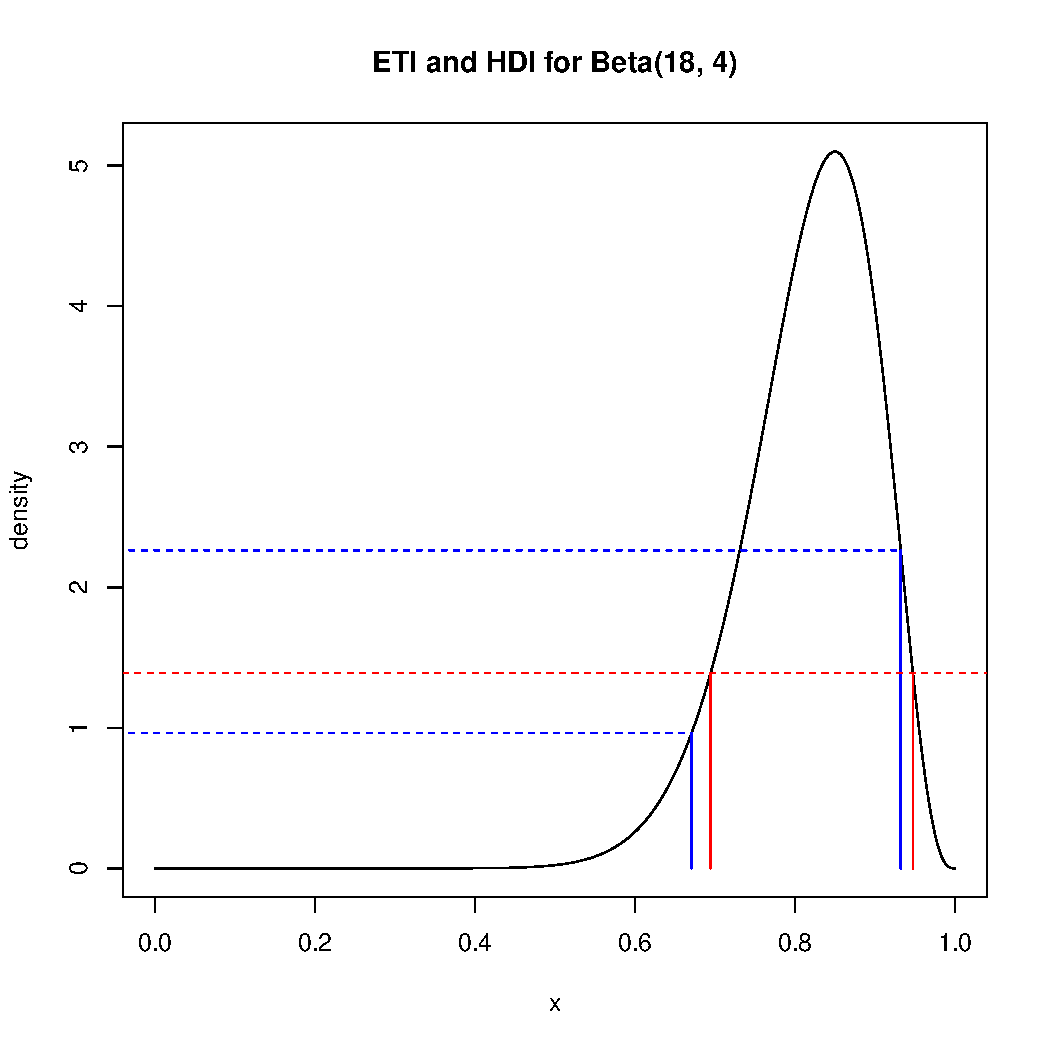
\includegraphics[width = 0.7\textwidth]{figs/eti_and_hdi}
  \caption{Comparison of 90\% ETI and HDI for Beta(18,4)}
  \label{fig:eti_and_hdi}
\end{figure}
Note that HDI can be hard to compute, a starting point of \mintinline{r}{R} script is shown here, using package
\mintinline{r}{bayestestR}:
\begin{minted}{r}
x <- seq(from = 0, to = 1, by = 0.001)
a <- 18
b <- 4
y1 <- dbeta(x, a, b)

# HDI
tmp <- bayestestR::distribution_beta(n = 100000, shape1 = a, shape2 = b)
tmp2 <- bayestestR::ci(tmp, ci = 0.90, method = "HDI")

# Compare HDI and SPI
bayestestR::ci(tmp, ci = 0.90, method = "HDI")
str(bayestestR::hdi(tmp, ci = 0.9))
str(bayestestR::spi(tmp, ci = 0.9))    # SPI is a more robust HDI
\end{minted}



\section{Predictive distribution}
\label{sec:pred-distr}

Note that if one wants to make some prediction/statement about $x$, like $x\in A$, then the probability can be computed as
\begin{equation}
  \label{eq:predictive_probability_definition}
    P\left(X \in A\right) = \int_A f_X\left(x\right)\mathrm{d}x
  = \int_A\int f_{X, \theta}\left(x, \theta\right)\mathrm{d}\theta\mathrm{d}x
  = \int_A\int f_{X|\theta}\left(x\middle|\theta\right)f_\theta\left(\theta\right)\mathrm{d}\theta\mathrm{d}x
  ,
\end{equation}
where $f_{X|\theta}\left(x\middle|\theta\right)$ is the data distribution and $f_\theta\left(\theta\right)$ is the distribution of $\theta$, either prior or posterior distribution. \eqref{eq:predictive_probability_definition} is called the \textbf{predictive probability} of $X\in A$, which is the probability based on marginal distribution of $X$.





\bibliographystyle{plainnat}
\bibliography{../ref}





\end{document}


%%% Local Variables:
%%% mode: latex
%%% TeX-master: t
%%% End:
